\begin{figure}[htbp]
\centering
\caption[A priori Sulfate Power Graph]{A priori Sulfate Power Graph}
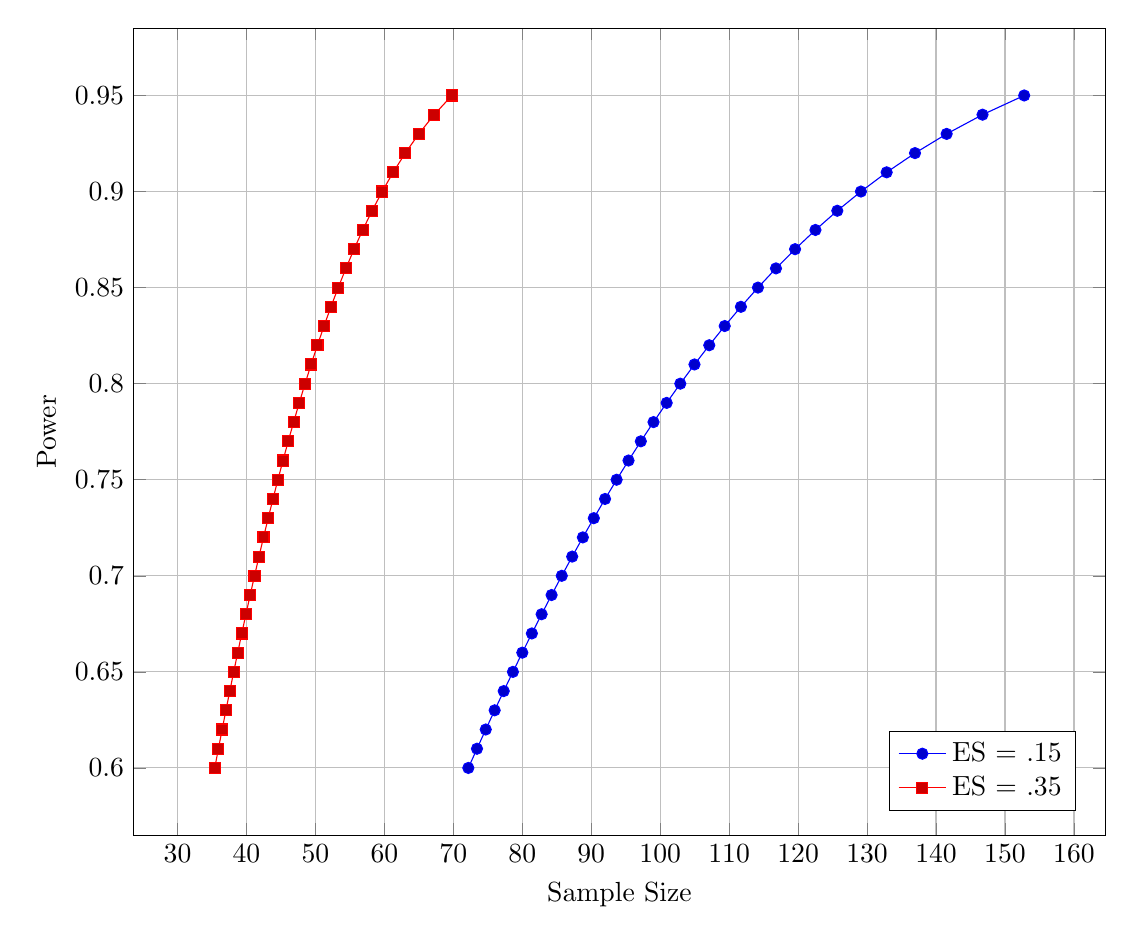
\begin{tikzpicture}
	\begin{axis}[grid=major,xlabel=Sample Size,ylabel=Power,scale=1.8, legend pos = south east] 
\addplot coordinates{
(72.1769,	0.60)
(73.4295,	0.61)
(74.701,	0.62)
(75.9928,	0.63)
(77.3061,	0.64)
(78.6423,	0.65)
(80.0031,	0.66)
(81.3899,	0.67)
(82.8048,	0.68)
(84.2495,	0.69)
(85.7262,	0.70)
(87.2373,	0.71)
(88.7853,	0.72)
(90.373,	0.73)
(92.0036,	0.74)
(93.6806,	0.75)
(95.4078,	0.76)
(97.1895,	0.77)
(99.0308,	0.78)
(100.937,	0.79)
(102.915,	0.80)
(104.971,	0.81)
(107.115,	0.82)
(109.356,	0.83)
(111.705,	0.84)
(114.177,	0.85)
(116.789,	0.86)
(119.559,	0.87)
(122.513,	0.88)
(125.683,	0.89)
(129.108,	0.90)
(132.84,	0.91)
(136.951,	0.92)
(141.538,	0.93)
(146.743,	0.94)
(152.786,	0.95)};
\addlegendentry{ES = .15}

\addplot coordinates{
(35.399	,0.60)
(35.932,	0.61)
(36.4731,	0.62)
(37.0229,	0.63)
(37.582,	0.64)
(38.1509,	0.65)
(38.7303,	0.66)
(39.321,	0.67)
(39.9236,	0.68)
(40.5391,	0.69)
(41.1683,	0.70)
(41.8122,	0.71)
(42.472,	0.72)
(43.1488,	0.73)
(43.8439,	0.74)
(44.5589,	0.75)
(45.2954,	0.76)
(46.0553,	0.77)
(46.8407,	0.78)
(47.6539,	0.79)
(48.4977,	0.80)
(49.3752,	0.81)
(50.29,	0.82)
(51.2464,	0.83)
(52.2493,	0.84)
(53.3046,	0.85)
(54.4195	,0.86)
(55.6024,	0.87)
(56.8641,	0.88)
(58.218,	0.89)
(59.6811,	0.90)
(61.2758,	0.91)
(63.0322,	0.92)
(64.9923,	0.93)
(67.2171,	0.94)
(69.8003,	0.95)};
\addlegendentry{ES = .35}


\end{axis}
\end{tikzpicture}
\label{fig:SulfatePowerGraph}
\end{figure}